\documentclass[landscape]{slides}
\usepackage[landscape, margin=2cm]{geometry}
\usepackage{color}
\usepackage{bm}
\usepackage{graphicx}
\usepackage{hyperref}
\graphicspath{ {./img/} }



\title{Sleep}
\author{Adam Johnson}
\date{30th April 2014}

\begin{document}

\maketitle


\begin{slide}

    \textcolor{blue}{\Large{Let's start with a personality quiz...}}

\end{slide}


\begin{slide}

    \textcolor{blue}{\Large{1) If you were free to plan your evening, and had no commitments the next day, what time would you choose to go to bed?}}

    \begin{enumerate}
        \item Before 21.00
        \item 21.00 - 22.30
        \item 22.30 - 00.00
        \item 00.00 - 01.30
        \item After 1.30
    \end{enumerate}

\end{slide}


\begin{slide}

    \textcolor{blue}{\Large{2) If you were free to plan your day, what time would choose to get up?}}

    \begin{enumerate}
        \item Before 06.30
        \item 06.30 - 08.00
        \item 08.00 - 09.30
        \item 09.300 - 11.00
        \item After 11.00
    \end{enumerate}

\end{slide}



\begin{slide}

    \textcolor{blue}{\Large{3) In general, do you find it easy to get up in the morning?}}

    \begin{enumerate}
        \item Definitely yes
        \item Yes
        \item Uncertain
        \item No
        \item Definitely no
    \end{enumerate}

\end{slide}



\begin{slide}

    \textcolor{blue}{\Large{4) Imagine that you have to do two hours of physically hard work. If you were entirely free to plan your day, in which of the following periods would you choose to do the work?}}

    \begin{enumerate}
        \item 08.00 - 11.00
        \item 11.00 - 13.00
        \item 13.00 - 15.00
        \item 15.00 - 17.00
        \item 17.00 - 19.00
    \end{enumerate}

\end{slide}



\begin{slide}

    \textcolor{blue}{\Large{Results...}}

    \begin{itemize}
        \item a
    \end{itemize}

\end{slide}


\begin{slide}

    \textcolor{blue}{\Large{Your Chronotype}}

    \begin{tabular}{c | c | c | c | c}

        4 - 6 &
        7 - 10 &
        11 - 13 &
        14 - 17 &
        18 - 20 \\

        \parbox[t]{4.2cm}{
            \begin{center}
            \textbf{Strong lark}
            \end{center}
        } &
        \parbox[t]{4.2cm}{
            \begin{center}
            \textbf{Moderate lark}
            \end{center}
        } &
        \parbox[t]{4.2cm}{
            \begin{center}
            \textbf{Neither owl nor lark}
            \end{center}
        } &
        \parbox[t]{4.2cm}{
            \begin{center}
            \textbf{Moderate owl}
            \end{center}
        } &
        \parbox[t]{4.2cm}{
            \begin{center}
            \textbf{Strong owl}
            \end{center}
        } \\

        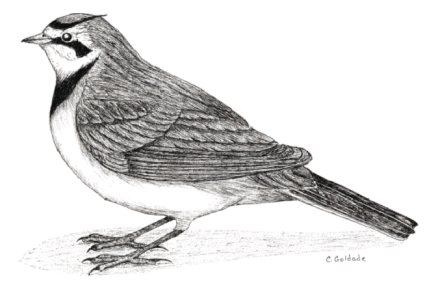
\includegraphics[width=4.2cm]{lark} &
        & & &
        
\includegraphics[width=4.2cm]{owl} \\

    \end{tabular}

\end{slide}



\begin{slide}

    \textcolor{blue}{\Large{What does your chronotype say about your personality?}}

    \textbf{Larks:}

    \begin{itemize}
        \item introverted, logical, and reliable
        \item get higher grades
    \end{itemize}

    \textbf{Owls:}

    \begin{itemize}
        \item extroverted, emotionally stable, hedonistic, and creative
        \item more likely to be obese
        \item average of four times as many partners during lifetime
    \end{itemize}

\end{slide}


% the time I spent in biphasic sleep

% Habits I've developed for sleep

    % go to bed alarm
    % Melatonin
    % yellow glasses
    % flux
    % naps


\begin{slide}

    \textcolor{blue}{\Large{Thanks!}}

    \begin{center}
        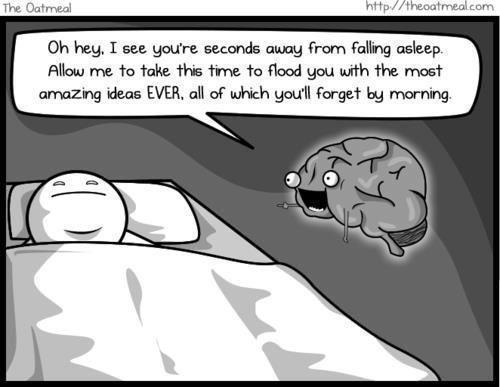
\includegraphics[height=15.5cm]{oatmeal-sleep-brain}
    \end{center}

\end{slide}


\end{document}
